\catcode`\~\active
\usepackage[pdftex]{graphicx}
\usepackage{tabularx}
\usepackage{times}
\usepackage[pdftex]{color}
\usepackage{rotating}
\definecolor{mygray}{gray}{0.75} 

\pagestyle{empty}

\setlength{\oddsidemargin}{0.0cm}
\setlength{\textwidth}{27.0cm}

\setlength{\topmargin}{0.0cm}
\setlength{\headheight}{0.0cm}
\setlength{\headsep}{0.0cm}
\setlength{\topskip}{0.0cm}
\setlength{\textheight}{20cm}

\setlength{\voffset}{-1.8cm}
\setlength{\hoffset}{-1.8cm}


\newcommand{\LI}{\setlength{\arrayrulewidth}{0.4mm}}
\newcommand{\li}{\setlength{\arrayrulewidth}{0.2mm}}
\setlength{\doublerulesep}{0mm}

\begin{document}
\parbox{10cm}{
\includegraphics[width=10cm]{\installpath/drache.png}}
\parbox[][][c]{7cm}{
\LI
  \begin{tabularx}{7.0cm}{|c|X|}\hline
\makebox[1.1cm]{Figur}&\namecharakter\\\hline
  \end{tabularx}

\vspace{2mm}\li
  \begin{tabularx}{7.0cm}{|c|X|}\hline
\makebox[1.1cm]{Spieler}&{\namespieler}\\\hline
  \end{tabularx}
}
\parbox{10cm}{\reflectbox{
\includegraphics[width=10cm]{\installpath/drache.png}}}

\vspace*{2ex}
\begin{minipage}[t]{13cm}
\LI
  \begin{tabular}[t]{|c|l|}\hline
\makebox[1.1cm]{\rule[-1.4ex]{0cm}{4ex}Typ}&\makebox[2.2cm]{\typ}\\\hline
  \end{tabular}
\hfill 
\li
  \begin{tabular}[t]{|c|l|}\hline
\makebox[1.1cm]{\rule[-1.4ex]{0cm}{4ex}\parbox[][][c]{1.1cm}{\renewcommand{\baselinestretch}{0}
\footnotesize Speziali"-sierung}}&\makebox[2.5cm]{{\spezialisierung}}\\\hline
  \end{tabular}\renewcommand{\baselinestretch}{1}
\hfill 
\LI
  \begin{tabular}[t]{|c|l|}\hline
\makebox[1.05cm]{\rule[-1.4ex]{0cm}{4ex}Grad}&\makebox[1.5cm]{{\grad}}\\\hline
  \end{tabular}

\vspace{1ex}
\li
  \begin{tabular}{|c|l|}\hline
\makebox[1.1cm]{\rule[-1.4ex]{0cm}{4ex}\small Herkunft}&\makebox[2.2cm]{\herkunft}\\\hline
  \end{tabular}
\hfill
\li
  \begin{tabular}{|c|l|}\hline
\makebox[1.1cm]{\rule[-1.4ex]{0cm}{4ex}Glaube}&\makebox[2.5cm]{\glaube}\\\hline
  \end{tabular}
\hfill
\li
  \begin{tabular}{|c|l|}\hline
\makebox[1.1cm]{\rule[-1.4ex]{0cm}{4ex}Stand}&\makebox[1.5cm]{\stand}\\\hline
  \end{tabular}

\vspace{1ex}
{\small
\begin{tabular}{|c|l|}\hline
Alter&\makebox[0.8cm]{{\alter}}\\\hline
\end{tabular}\hfill
\begin{tabular}{|c|l|}\hline
Gestalt&\makebox[0.8cm]{\gestalt}\\\hline
\end{tabular}\hfill
\begin{tabular}{|c|l|}\hline
Gewicht&\makebox[0.8cm]{\gewicht}\\\hline
\end{tabular}\hfill
\begin{tabular}{|c|l|}\hline
K�rpergr��e&\makebox[0.8cm]{\koerpergroesse}\\\hline
\end{tabular}

\vspace{1ex}
\renewcommand{\arraystretch}{0.9}

\begin{tabular}{|c|c|}\hline
Beruf&\makebox[1.5cm]{\beruf}\\\hline
\end{tabular}
\hfill
\begin{tabular}{|c|c|}\hline
Hand&\makebox[1.2cm]{\hand}\\\hline
\end{tabular}
\hfill
\begin{tabular}{|c|c|}\hline
Spezies&\makebox[1.2cm]{\spezies}\\\hline
\end{tabular}

\begin{tabularx}{13cm}{|c|X|}\hline
\raisebox{-0.3ex}[0.3ex]{weitere}&{\merkmale}\\
\raisebox{0.3ex}[-0.3ex]{Merkmale}\rule[-1ex]{0ex}{3.3ex}&\\\hline
\end{tabularx}\renewcommand{\arraystretch}{1}
}

\vspace{1ex}
\normalsize
\LI
\begin{tabular}{|c|c|}\hline
\makebox[0.6cm]{St}&\makebox[0.6cm]{{\st}}\\\hline
\end{tabular}\hfill
\begin{tabular}{|c|c|}\hline
\makebox[0.6cm]{Ko}&\makebox[0.6cm]{{\ko}}\\\hline
\end{tabular}\hfill
\li
\begin{tabular}{|c|c|}\hline
\makebox[0.6cm]{Au}&\makebox[0.6cm]{{\au}}\\\hline
\end{tabular}\hfill
\begin{tabular}{|c|c|}\hline
\makebox[0.6cm]{Sb}&\makebox[0.6cm]{{\sbb}}\\\hline
\end{tabular}\hfill
\begin{tabular}{|c|c|}\hline
\makebox[0.6cm]{KAW}&\makebox[0.6cm]{{\kaw}}\\\hline
\end{tabular}

\vspace{1ex}
\LI
\begin{tabular}{|c|c|}\hline
\makebox[0.6cm]{Gs}&\makebox[0.6cm]{{\gs}}\\\hline
\end{tabular}\hfill
\begin{tabular}{|c|c|}\hline
\makebox[0.6cm]{In}&\makebox[0.6cm]{{\inn}}\\\hline
\end{tabular}\hfill
\li
\begin{tabular}{|c|c|}\hline
\makebox[0.6cm]{pA}&\makebox[0.6cm]{{\pa}}\\\hline
\end{tabular}\hfill
\begin{tabular}{|c|c|}\hline
\makebox[0.6cm]{Wk}&\makebox[0.6cm]{{\wk}}\\\hline
\end{tabular}\hfill
\begin{tabular}{|c|c|}\hline
\makebox[0.6cm]{\tiny Geistesblitz}&\makebox[0.6cm]{{\geistesblitz}}\\\hline
\end{tabular}

\vspace{1ex}
\LI
\begin{tabular}{|c|c|}\hline
\makebox[0.6cm]{Gw}&\makebox[0.6cm]{{\gw}}\\\hline
\end{tabular}\hfill
\begin{tabular}{|c|c|}\hline
\makebox[0.6cm]{Zt}&\makebox[0.6cm]{{\zt}}\\\hline
\end{tabular}\hfill
\li
\begin{tabular}{|c|c|}\hline
\makebox[0.6cm]{B}&\makebox[0.6cm]{{\bb}}\\\hline
\end{tabular}\hfill
\begin{tabular}{|c|c|}\hline
\makebox[0.6cm]{GG}&\makebox[0.6cm]{{\ggn}}\\\hline
\end{tabular}\hfill
\begin{tabular}{|c|c|}\hline
\makebox[0.6cm]{SG}&\makebox[0.6cm]{\sg}\\\hline
\end{tabular}

\vspace{1ex}
%\IfFileExists{MAGUS-Logo-grey2.png}{\parbox{1.5cm}{\includegraphics[width=1.5cm]{MAGUS-Logo-grey2.png}}}%
%\parbox{1.cm}{\includegraphics[width=1.5cm]{\installpath/MAGUS-Logo-grey2.png}}
%\hfill
\parbox[t]{2.8cm}{
~\\
\tiny
\begin{tabular}{|l|c|l|r|}
\hline
\multicolumn{2}{|l|}{pers. Boni f�r} \\\hline
Ausdauer      & \boau    \\
Schaden       & \bosc    \\
Angriff       & \boan    \\
Abwehr        & \boab    \\
Zaubern       & \boza    \\
Geistesmagie  & \bopsy   \\
K�rpermagie   & \bophs   \\
Umgebungsmagie& \bophk   \\\hline
\end{tabular}
}
%\hfill
\parbox[t]{5cm}{
~\\
\footnotesize
\begin{tabular}{|l|r|l|}
\hline
GFP    & \makebox[0.8cm]{\gfp}  &\hspace{2cm}  \\\hline
KEP    & \kep  &  \\\hline
ZEP    & \zep  &  \\\hline
AEP    & \aep  &  \\\hline
\end{tabular}

\hspace*{1.0cm} {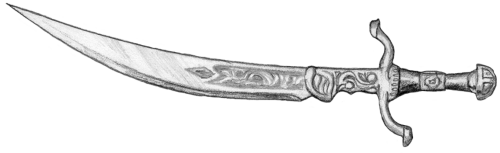
\includegraphics[height=0.7cm,angle=0]{\installpath/saebel.png}}
}
%\hfill
\parbox[t]{4.9cm}{
~\\
\footnotesize
\begin{tabular}{|l|r|l|}
\hline
Gold   &  \makebox[0.8cm]{\gold}   &\hspace{2cm}  \\\hline 
Silber & \silber &  \\\hline             
Kupfer & \kupfer &  \\\hline             
\end{tabular}

\hfill {
\includegraphics[height=1.2cm,angle=0]{\installpath/Money-gray.png}}
}
\hfill
%\IfFileExists{wurfbeil.png}{\parbox{2cm}{\includegraphics[width=2cm]{wurfbeil.png}}}%
%\parbox{2cm}{\includegraphics[width=2cm]{\installpath/wurfbeil.png}}
%\parbox{2cm}{
\includegraphics[width=2cm]{\installpath/Letter-Feather-grey.png}}
%\hfill~

\parbox{6cm}
{
\vspace{1ex}\LI
\begin{tabularx}{5.9cm}{|p{0.5cm}|c|X|}\hline
\makebox[0.4cm]{LP}&\makebox[0.4cm]{{\lp}}&\\\hline
\makebox[0.4cm]{AP}&\makebox[0.4cm]{{\ap}}&\\\hline
\end{tabularx}

\parbox{3.3cm}{
\li
\vspace*{1ex}
{\setlength{\tabcolsep}{0.3em}
\footnotesize
\begin{tabular}{|l|c|}
\hline
\multicolumn{2}{|l|}{Sinne}\\\hline
Sehen          & \sinnse   \\
H�ren          & \sinnh    \\
Riechen        & \sinnr    \\
Schmecken      & \sinnsc   \\
Tasten         & \sinnt    \\
Sechster Sinn  & \sinnss   \\\hline
\multicolumn{2}{l}{}\\\hline
\multicolumn{2}{|l|}{Erfolgswerte}\\\hline
Abwehr        & \abwehr \\
Zaubern       & \zauber \\\hline
\multicolumn{2}{l}{}\\\hline
\multicolumn{2}{|l|}{Resistenzen}\\\hline
Gift          & \gift   \\
Resistenz     & \res    \\
Geistesmagie  & \psy    \\
K�rpermagie   & \phs    \\
Umgebungsmagie& \phk    \\\hline
\end{tabular}
}
%\begin{tabular}{|c@{\LI\hspace*{1.4ex}\vline\hspace*{1.4ex}}c@{\LI\hspace*{1.4ex}\vline\hspace*{1.4ex}}c|c|c|c|} \hline
%Datum\hspace*{2.5em}&GFP&KEP&ZEP&AEP&Geld\\\hline\hline
%&{\gfp}&{\kep}&{\zep}&{\aep}&{\gold}\\\hline
%&&&&&\\\hline
%&&&&&\\\hline
%&&&&&\\\hline
%&&&&&\\\hline
%&&&&&\\\hline
%&&&&&\\\hline
%&&&&&\\\hline
%&&&&&\\\hline
%&&&&&\\\hline
%&&&&&\\\hline
%&&&&&\\\hline
%&&&&&\\\hline
%&&&&&\\\hline
%&&&&&\\\hline
%&&&&&\\\hline
%&&&&&\\\hline
%&&&&&\\\hline
%&&&&&\\\hline
%\end{tabular}
}
%\parbox{2.5cm}{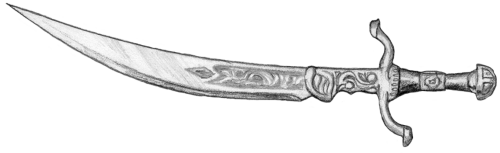
\includegraphics[height=1.7cm,angle=280]{\installpath/saebel.png}}
\parbox{2.5cm}{

\includegraphics[width=2.5cm]{\installpath/Letter-Feather-grey.png}
%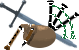
\includegraphics[width=2.5cm]{\installpath/Alba-grey.png}
%\vspace{1.cm}

%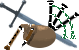
\includegraphics[width=2.5cm]{\installpath/Alba-grey.png}
\parbox{0.5cm}{\includegraphics[width=2.5cm]{\installpath/MAGUS-Logo-grey2.png}}
%\includegraphics[width=2.5cm]{\installpath/wurfbeil.png}
}
}
\parbox[t]{7cm}
{\setlength{\tabcolsep}{0.5em}
\scriptsize
\begin{tabular}{|p{2.6cm}|c|p{2.6cm}|}
  \hline
Sprache&Wert&Schrift\\\hline\hline
{\spraa}&{\sprawa}&{\schra}\\\hline
{\sprab}&{\sprawb}&{\schrb}\\\hline
{\sprac}&{\sprawc}&{\schrc}\\\hline
{\sprad}&{\sprawd}&{\schrd}\\\hline
{\sprae}&{\sprawe}&{\schre}\\\hline
{\spraf}&{\sprawf}&{\schrf}\\\hline
{\sprag}&{\sprawg}&{\schrg}\\\hline
{\sprah}&{\sprawh}&{\schrh}\\\hline
{\sprai}&{\sprawi}&{\schri}\\\hline
{\spraj}&{\sprawj}&{\schrj}\\\hline
{\sprak}&{\sprawk}&{\schrk}\\\hline
{\spral}&{\sprawl}&{\schrl}\\\hline
{\spram}&{\sprawm}&{\schrm}\\\hline
{\spran}&{\sprawn}&{\schrn}\\\hline
{\sprao}&{\sprawo}&{\schro}\\\hline
{\sprap}&{\sprawp}&{\schrp}\\\hline
{\spraq}&{\sprawq}&{\schrq}\\\hline
{\sprar}&{\sprawr}&{\schrr}\\\hline
{\spras}&{\spraws}&{\schrs}\\\hline
{\sprat}&{\sprawt}&{\schrt}\\\hline
{\sprau}&{\sprawu}&{\schru}\\\hline
{\sprav}&{\sprawv}&{\schrv}\\\hline
{\spraw}&{\spraww}&{\schrw}\\\hline
\end{tabular} 
}
\end{minipage}
\hspace{3ex}
\begin{minipage}[t]{5.4cm}
\setlength{\tabcolsep}{0.4em}
\footnotesize
    \begin{tabular}[t]{|p{4cm}|c|r|}\hline
      \multicolumn{3}{|c|}{\small angeborene und erlernte}\\
      \multicolumn{3}{|c|}{\small F�higkeiten und Waffenfertigkeiten}\\[1ex]
      \normalsize Fertigkeit&{$\!$\normalsize PP$\!$}&{$\!\!$\normalsize EW$\!\!$}\\\hline\hline
\makebox[4cm][l]{\ferta }      &{\praxisa }&{\werta }\\\hline
\makebox[4cm][l]{\fertb }      &{\praxisb }&{\wertb }\\\hline
\makebox[4cm][l]{\fertc }      &{\praxisc }&{\wertc }\\\hline
\makebox[4cm][l]{\fertd }      &{\praxisd }&{\wertd }\\\hline
\makebox[4cm][l]{\ferte }      &{\praxise }&{\werte }\\\hline
\makebox[4cm][l]{\fertf }      &{\praxisf }&{\wertf }\\\hline
\makebox[4cm][l]{\fertg }      &{\praxisg }&{\wertg }\\\hline
\makebox[4cm][l]{\ferth }      &{\praxish }&{\werth }\\\hline
\makebox[4cm][l]{\ferti }      &{\praxisi }&{\werti }\\\hline
\makebox[4cm][l]{\fertj }      &{\praxisj }&{\wertj }\\\hline
\makebox[4cm][l]{\fertk }      &{\praxisk }&{\wertk }\\\hline
\makebox[4cm][l]{\fertl }      &{\praxisl }&{\wertl }\\\hline
\makebox[4cm][l]{\fertm }      &{\praxism }&{\wertm }\\\hline
\makebox[4cm][l]{\fertn }      &{\praxisn }&{\wertn }\\\hline
\makebox[4cm][l]{\ferto }      &{\praxiso }&{\werto }\\\hline
\makebox[4cm][l]{\fertp }      &{\praxisp }&{\wertp }\\\hline
\makebox[4cm][l]{\fertq }      &{\praxisq }&{\wertq }\\\hline
\makebox[4cm][l]{\fertr }      &{\praxisr }&{\wertr }\\\hline
\makebox[4cm][l]{\ferts }      &{\praxiss }&{\werts }\\\hline
\makebox[4cm][l]{\fertt }      &{\praxist }&{\wertt }\\\hline
\makebox[4cm][l]{\fertu }      &{\praxisu }&{\wertu }\\\hline
\makebox[4cm][l]{\fertv }      &{\praxisv }&{\wertv }\\\hline
\makebox[4cm][l]{\fertw }      &{\praxisw }&{\wertw }\\\hline
\makebox[4cm][l]{\fertx }      &{\praxisx }&{\wertx }\\\hline
\makebox[4cm][l]{\ferty }      &{\praxisy }&{\werty }\\\hline
\makebox[4cm][l]{\fertz }      &{\praxisz }&{\wertz }\\\hline
\makebox[4cm][l]{\fertaa}      &{\praxisaa}&{\wertaa}\\\hline
\makebox[4cm][l]{\fertab}      &{\praxisab}&{\wertab}\\\hline
\makebox[4cm][l]{\fertac}      &{\praxisac}&{\wertac}\\\hline
\makebox[4cm][l]{\fertad}      &{\praxisad}&{\wertad}\\\hline
\makebox[4cm][l]{\fertae}      &{\praxisae}&{\wertae}\\\hline
\makebox[4cm][l]{\fertaf}      &{\praxisaf}&{\wertaf}\\\hline
\makebox[4cm][l]{\fertag}      &{\praxisag}&{\wertag}\\\hline
\makebox[4cm][l]{\fertah}      &{\praxisah}&{\wertah}\\\hline
\makebox[4cm][l]{\fertai}      &{\praxisai}&{\wertai}\\\hline
\makebox[4cm][l]{\fertaj}      &{\praxisaj}&{\wertaj}\\\hline
\makebox[4cm][l]{\fertak}      &{\praxisak}&{\wertak}\\\hline
\makebox[4cm][l]{\fertal}      &{\praxisal}&{\wertal}\\\hline
\makebox[4cm][l]{\fertam}      &{\praxisam}&{\wertam}\\\hline
\makebox[4cm][l]{\fertan}      &{\praxisan}&{\wertan}\\\hline
    \end{tabular}
\end{minipage}
\hspace{2ex}
%\fbox{
\begin{minipage}[t]{7.5cm}
%\small
\scriptsize
\setlength{\tabcolsep}{0.3em}
    \begin{tabular}[t]{||p{3.1cm}|c|c||}\hline\hline
%      \raisebox{-1ex}[2ex][0ex]{\LARGE Waffe}&\normalsize Erfolgswert&\footnotesize Waffenrang\\\cline{2-3}
      \normalsize Waffe &\normalsize Erfolgswert&\footnotesize Waffenrang\\\cline{2-3}
%      \raisebox{-0.2ex}[1ex][0.2ex]{\footnotesize (Reichweite)}&\normalsize\raisebox{-0.2ex}[1ex][0.2ex]{Schaden}&\footnotesize Abwehrmod.\\\hline\hline\hline
      \scriptsize (Reichweite)&\normalsize\raisebox{-0.2ex}[1ex][0.2ex]{Schaden}&\footnotesize Abwehrmod.\\\hline\hline\hline
      &{\waffeEa}&{\waffeAa}\\\cline{2-3}
      \raisebox{1.5ex}[-1.5ex]{\makebox[2cm][l]{{\waffea}}}&{\waffeSa}&{\waffeVa}\\\hline\hline
      &{\waffeEb}&{\waffeAb}\\\cline{2-3}
      \raisebox{1.5ex}[-1.5ex]{\makebox[2cm][l]{{\waffeb}}}&{\waffeSb}&{\waffeVb}\\\hline\hline
      &{\waffeEc}&{\waffeAc}\\\cline{2-3}
      \raisebox{1.5ex}[-1.5ex]{\makebox[2cm][l]{{\waffec}}}&{\waffeSc}&{\waffeVc}\\\hline\hline
      &{\waffeEd}&{\waffeAd}\\\cline{2-3}
      \raisebox{1.5ex}[-1.5ex]{\makebox[2cm][l]{{\waffed}}}&{\waffeSd}&{\waffeVd}\\\hline\hline
      &{\waffeEe}&{\waffeAe}\\\cline{2-3}
      \raisebox{1.5ex}[-1.5ex]{\makebox[2cm][l]{{\waffee}}}&{\waffeSe}&{\waffeVe}\\\hline\hline
      &{\waffeEf}&{\waffeAf}\\\cline{2-3}
      \raisebox{1.5ex}[-1.5ex]{\makebox[2cm][l]{{\waffef}}}&{\waffeSf}&{\waffeVf}\\\hline\hline
      &{\waffeEg}&{\waffeAg}\\\cline{2-3}
      \raisebox{1.5ex}[-1.5ex]{\makebox[2cm][l]{{\waffeg}}}&{\waffeSg}&{\waffeVg}\\\hline\hline
      &{\waffeEh}&{\waffeAh}\\\cline{2-3}
      \raisebox{1.5ex}[-1.5ex]{\makebox[2cm][l]{{\waffeh}}}&{\waffeSh}&{\waffeVh}\\\hline\hline
      &{\waffeEi}&{\waffeAi}\\\cline{2-3}
      \raisebox{1.5ex}[-1.5ex]{\makebox[2cm][l]{{\waffei}}}&{\waffeSi}&{\waffeVi}\\\hline\hline
      &{\waffeEj}&{\waffeAj}\\\cline{2-3}
      \raisebox{1.5ex}[-1.5ex]{\makebox[2cm][l]{{\waffej}}}&{\waffeSj}&{\waffeVj}\\\hline\hline
      &{\waffeEk}&{\waffeAk}\\\cline{2-3}
      \raisebox{1.5ex}[-1.5ex]{\makebox[2cm][l]{{\waffek}}}&{\waffeSk}&{\waffeVk}\\\hline\hline
      &{\waffeEl}&{\waffeAl}\\\cline{2-3}
      \raisebox{1.5ex}[-1.5ex]{\makebox[2cm][l]{{\waffel}}}&{\waffeSl}&{\waffeVl}\\\hline\hline
    \end{tabular}

\vspace{1ex}
\parbox{5cm}{
{
\Li
\scriptsize
%\hfill
%\setlength{\tabcolsep}{0.3ex}
%    \begin{tabular}{|l|c|c|l|c|} \cline{1-2}\cline{4-5}
%\rule[-0.2ex]{0cm}{3.0ex} ~R�stungsklasse & \makebox[3em]{\ruestung/\ruestungb}             &\hspace*{1em} & ~Abwehr         & \abwehrfinal \\\cline{1-2}\cline{4-5}
%\rule[-0.2ex]{0cm}{3.0ex} ~Schutz vor LP--Verlust &\makebox[3em]{~\ruestunglp/\ruestunglpb}  &              &  ~mit Verteidigungswaffe& \abwehrmitwaffe\\\cline{1-2}\cline{4-5}
    \begin{tabular}{|||l|c|||} \hline\hline\hline
\rule[-0.2ex]{0cm}{3.0ex} R�stungsklassen & \ruestung/\ruestungb \\\hline
\rule[-0.2ex]{0cm}{3.0ex} Schutz vor LP--Verlust &\ruestunglp/\ruestunglpb \\\hline\hline
\rule[-0.2ex]{0cm}{3.0ex} Abwehr         & \abwehrfinal \\\hline
\rule[-0.2ex]{0cm}{3.0ex} mit Verteidigungswaffe& \abwehrmitwaffe\\\hline\hline\hline
   \end{tabular}
%\hfill
}

\vspace{1ex}
%\parbox{7.5cm}{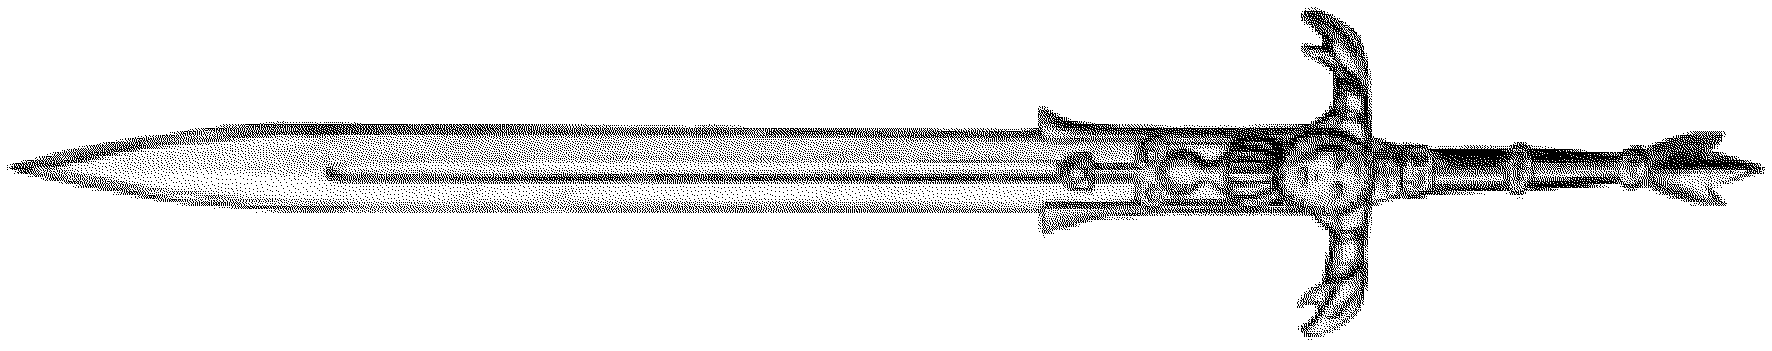
\includegraphics[width=7.5cm]{\installpath/schwert.png}}
% \vspace*{2ex}

%\vspace{-2.5ex}
\scalebox{0.7}{
\parbox{7.7cm}
{
 \footnotesize
\setlength{\tabcolsep}{0.2em}\renewcommand{\arraystretch}{0.8}
    \begin{tabular}[b]{l|l|l|l|l|l|l}
      \multicolumn{4}{l}{\small Grundkenntnisse in}\\\cline{2-2}\cline{4-4}\cline{6-6}   
      Einhandschwert     &\makebox[1ex]{\usebox{\Einhandschwert}} & Stichwaffe  &\makebox[1ex]{\usebox{\Stichwaffe}}                & Armbrust    &\makebox[1ex]{\usebox{\Armbrust}}                   \\\cline{2-2}\cline{4-4}\cline{6-6}   
      Einhandschlagwaffe &\usebox{\Einhandschlagwaffe}            & Spie�waffe  &\usebox{\Spiesswaffe}               & Bogen       &\usebox{\Bogen}                      \\\cline{2-2}\cline{4-4}\cline{6-6}
      Zweihandschwert    &\usebox{\Zweihandschwert}               & Kettenwaffe &\usebox{\Kettenwaffe}               & Schleuder   &\usebox{\Schleuder}                  \\\cline{2-2}\cline{4-4}\cline{6-6}
      Zweihandschlagwaffe&\usebox{\Zweihandschlagwaffe}           & Fesselwaffe &\usebox{\Fesselwaffe}               & Wurfscheibe &\usebox{\Wurfscheibe}                \\\cline{2-2}\cline{4-4}\cline{6-6}
      Kampf ohne Waffen  &\usebox{\KampfohneWaffen}               & Zauberst�be &\usebox{\Zauberstaebe}              & Wurfspie�   &\makebox[1ex]{\usebox{\Wurfspiess}}  \\\cline{2-2}\cline{4-4}\cline{6-6}
      Stangenwaffe       &\usebox{\Stangenwaffe}                  & Schild      &\usebox{\Schild}                  \\\cline{2-2}\cline{4-4}
      Stielwurfwaffe     &\usebox{\Stielwurfwaffe}                & Parierwaffe &\usebox{\Parierwaffe}             \\\cline{2-2}\cline{4-4}
    \end{tabular}
}
}
}
\hspace{-3.3em}\fbox{\parbox{0.5cm}{\includegraphics[width=3.5cm]{\installpath/wurfbeil.png}}}



%\vspace{3.5ex}
%\vfill
\parbox{7.5cm}
{\renewcommand{\arraystretch}{0.7}
\tiny
\begin{tabular}{|lrlrlr|}
\hline
\multicolumn{6}{|c|}{\footnotesize \rule[-0.0ex]{0cm}{2.ex}Ungelernte Fertigkeiten}\\\hline
\unia  & \uniwa  & \uniq  & \uniwq  & \uniag & \uniwag\\
\unib  & \uniwb  & \unir  & \uniwr  & \uniah & \uniwah\\
\unic  & \uniwc  & \unis  & \uniws  & \uniai & \uniwai\\
\unid  & \uniwd  & \unit  & \uniwt  & \uniaj & \uniwaj\\
\unie  & \uniwe  & \uniu  & \uniwu  & \uniak & \uniwak\\
\unif  & \uniwf  & \univ  & \uniwv  & \unial & \uniwal\\
\unig  & \uniwg  & \uniw  & \uniww  & \uniam & \uniwam\\
\unih  & \uniwh  & \unix  & \uniwx  & \unian & \uniwan\\
\unii  & \uniwi  & \uniy  & \uniwy  & \uniao & \uniwao\\
\unij  & \uniwj  & \uniz  & \uniwz  & \uniap & \uniwap\\
\unik  & \uniwk  & \uniaa & \uniwaa & \uniaq & \uniwaq\\
\unil  & \uniwl  & \uniab & \uniwab & \uniar & \uniwar\\
\unim  & \uniwm  & \uniac & \uniwac & \unias & \uniwas\\
\unin  & \uniwn  & \uniad & \uniwad & \uniat & \uniwat\\
\unio  & \uniwo  & \uniae & \uniwae & \uniau & \uniwau\\
\unip  & \uniwp  & \uniaf & \uniwaf & \uniav & \uniwav\\\hline
\end{tabular}}

\tiny\hfill\today
\end{minipage}


